%%%%%%%%%%%%%%%%%%%%%%%%%%%%%%%%%%%%%%%%%%%%%%%%%%%%%%%%%%%%%%%%%%%%%%
%%%%%                                                                %
%%%%% Document Class                                                 %
%%%%%                                                                %
%%%%%%%%%%%%%%%%%%%%%%%%%%%%%%%%%%%%%%%%%%%%%%%%%%%%%%%%%%%%%%%%%%%%%%
\documentclass{beamer}

%%%%% Package loading
\usepackage[utf8]{inputenc}
\usepackage[english]{babel}
\usepackage[T1]{fontenc}

\usepackage{lmodern}
\usepackage{xcolor}
\usepackage{listings}

\usepackage{makecell}

% Tikz/plots
\usepackage{tikz}
\usetikzlibrary{backgrounds}
\usepackage{pgfplots}
\usetikzlibrary{pgfplots.groupplots}

\pgfplotscreateplotcyclelist{mylist}{ 
  fill=gray!20,draw=black!90,line width=.2pt\\%
  fill=blue!60,draw=black!90,line width=.2pt\\%
  fill=red!60,draw=black!90,line width=.2pt\\%
  fill=orange!60,draw=black!90,line width=.2pt\\%
  fill=yellow!60,draw=black!90,line width=.2pt\\%
  fill=green!60,draw=black!90,line width=.2pt\\%
  fill=white\\%
}

\definecolor{hiBlue}{HTML}{0069B4}

\newcommand\drawbar[1]{%
  \begin{tikzpicture}%
    \draw[fill=#1,draw=black!90,ultra thin] (0pt,0pt) rectangle (3pt,8pt);%
    \draw[fill=#1,draw=black!90,ultra thin] (6pt,0pt) rectangle (9pt,6pt);%
  \end{tikzpicture}\hspace{0pt}%
}

%%%%% IIS theme-specific settings.
\usetheme[%
% waferpng %% Use the PNG version of the wafer image on the title slide (increases file size!).
]{iis}

%% (Optional) Scale the wafer image on the title page.
\setwaferwidth{0.5} % In percent of the \linewidth (default: 0.5)
\setwaferleft{0.0}  % In centimeter from the top-left corner of the slide (default: 0.0)
\setwafertop{5.8}   % In centimeter from the top-left corner of the slide (default: 5.8)

%% (Optional) Change the margin of the text on the slides (default =
%% 2em). Note that we currently do not adapt the indentation of the
%% frametitle accordingly.
% \setbeamersize{text margin left=1em, text margin right=1em}

%% You may change the appearance of the navigation symbols (shown at
%% the bottom right of each slide) using any of the following lines.
% \setbeamertemplate{navigation symbols}{} %% Disable navigation symbols
% \setbeamertemplate{navigation symbols}[vertical] %% Vertically organize the navigation symbols.
% \setbeamertemplate{navigation symbols}[only frame symbol] %% Only show frame symbols


%%%%% Settings, specific only for this presentation.
\newcommand\latexcls[1]{\textsf{#1}}
\newcommand\latexsty[1]{\textsf{#1}}

%% A listing style for LaTeX/TeX code (note that the colors being used
%% are defined in the iis beamer template).
\lstdefinestyle{latexcodestyle}{
  basicstyle        = \ttfamily,              %% The basic font style to be used for the code
  keywordstyle      = \color{eth4}\bfseries,  %% The keyword style
  language          = {[LaTeX]TeX},           %% The language of the code
  texcsstyle        = *\color{eth7}\bfseries, %% Style of LaTeX/TeX-specific code
  moretexcs         = {usetheme},             %% Additional LaTeX/TeX-specifc keywords
  morekeywords      = {iis},                  %% Other keywords
}


\newcommand{\beginbackup}{
   \newcounter{framenumbervorappendix}
   \setcounter{framenumbervorappendix}{\value{framenumber}}
}
\newcommand{\backupend}{
   \addtocounter{framenumbervorappendix}{-\value{framenumber}}
   \addtocounter{framenumber}{\value{framenumbervorappendix}}
}


%%%%%%%%%%%%%%%%%%%%%%%%%%%%%%%%%%%%%%%%%%%%%%%%%%%%%%%%%%%%%%%%%%%%%%
%%%%%                                                                %
%%%%% Document Settings                                              %
%%%%%                                                                %
%%%%%%%%%%%%%%%%%%%%%%%%%%%%%%%%%%%%%%%%%%%%%%%%%%%%%%%%%%%%%%%%%%%%%%

\title{OpenRISC Instruction Set Architecture Extensions}
\subtitle{Master Thesis}
\date{Zurich, May 2015}

%% Determine the authors of the work.
\author[%
  Andreas Traber %% Used for the footline.
]{%
  \textbf{Andreas Traber} \\%% The author giving the presentation.
  \vspace{2em}
  \textbf{Advisors}\\
  Michael Gautschi\\
  Antonio Pullini \\
  Prof. Dr. Luca Benini \\
  \vfill%% Any further authors should come in here.
}

\institute[%
  Integrated Systems Laboratory%% The short version of the institute will be used for the footer.
]{Integrated Systems Laboratory}

\setcounter{tocdepth}{1}


%%%%%%%%%%%%%%%%%%%%%%%%%%%%%%%%%%%%%%%%%%%%%%%%%%%%%%%%%%%%%%%%%%%%%%
%%%%%                                                                %
%%%%% Document Start                                                 %
%%%%%                                                                %
%%%%%%%%%%%%%%%%%%%%%%%%%%%%%%%%%%%%%%%%%%%%%%%%%%%%%%%%%%%%%%%%%%%%%%
\begin{document}


\begin{frame}[%
  plain, %% We do not want to have headers and footers on the title page.
  noframenumbering, %% Do not consider the title page for frame numbers.
]
\titlepage
\end{frame}

\begin{frame}
  \frametitle{Outline}
  \tableofcontents
\end{frame}

\section{Motivation}
\subsection{Motivation}

\begin{frame}
  \frametitle{Motivation}
  \framesubtitle{Ultra-Low-Power Computing}
  \vfill
  \begin{itemize}
    \item Todays embedded devices need a vast amount of computing power \\
      {\color{gray}Internet of things, wearable devices, sensors, smartphones,
      \ldots}

    \item Need to be energy efficient\\
      {\color{gray}Operate digital circuits near the threshold voltage}

    \item Use parallelization to recover performance\\
      {\color{gray}Turn off unused processing elements}\\
      \vspace{1.5em}
    \centering\includegraphics<1>[height=0.40\textheight]{figures/near_threshold}
  \end{itemize}
\end{frame}

\subsection{PULP}

\begin{frame}
  \frametitle{PULP}
  \framesubtitle{Parallel Ultra-Low power Processor}
  \centering\includegraphics<1>[width=1.0\textwidth]{figures/PULP_PE.png}
  \centering\includegraphics<2>[width=1.0\textwidth]{figures/PULP_PE2.png}
  \begin{itemize}
    \item<2> My work is focused on the PE
  \end{itemize}
\end{frame}

\subsection{OR10N}

\begin{frame}
  \frametitle{PE: OR10N}
  \framesubtitle{In-order 4-stage OpenRISC CPU}
  \vfill
  \centering\includegraphics<1>[width=1.0\textwidth]{figures/or10n_overview}
\end{frame}

\subsection{Goals}

\begin{frame}
  \frametitle{Goals}
  \begin{itemize}
    \item Higher energy efficiency
    %
    \vfill
    %
    \uncover<2->{
    \item Doing more computations per cycle $\Rightarrow$ ISA extensions
      \begin{itemize}
        \item {\color{gray}Hardware loops
        \item Auto-incrementing load/stores}
        \item Vectorial instructions
        \item Improved MAC
        \item Bit counting instructions
      \end{itemize}
    }
    %
    \vfill
    \item<3-> No increase in clock cycle time
    %
    \vfill
    %
    \uncover<4->{
    \item Extensions supported by compiler \\
         {\color{gray}New instructions generated automatically}
    }
    %
    \vfill
  \end{itemize}
\end{frame}




\section{Vectorial ALU}

\begin{frame}
  \frametitle{Vectorial ALU}
  \framesubtitle{Use subword parallelism}
  \begin{itemize}
    \item Re-use existing ALU and data path
    \item Segment the data path dynamically into 2/4 parts
    \item No separate register file needed
    \uncover<2>{
    \item Unaligned memory access \\
          \vfill
          \centering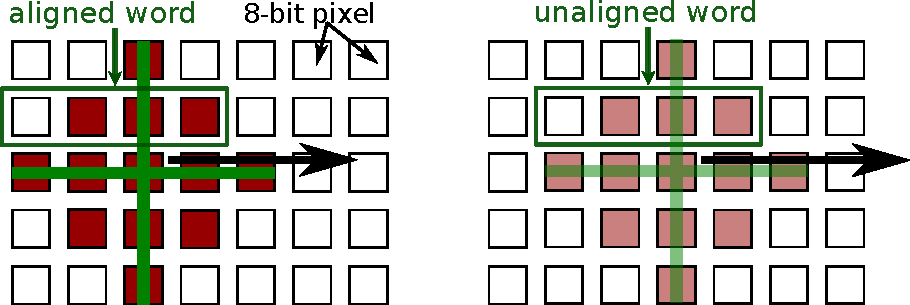
\includegraphics[width=0.8\textwidth]{figures/unaligned_mem_access_5x5}
    }
  \end{itemize}
  %
  \vfill
  %
\end{frame}


\begin{frame}
  \frametitle{Vectorial ALU}
  \framesubtitle{Encoding}
  %
  \begin{center}
    \includegraphics[width=0.8\textwidth]{figures/encoding}
  \end{center}
  %
  \vspace{10pt}
  %
  \begin{itemize}
    \item Sub-opcodes
  \end{itemize}

  \hspace{10pt}
  \begin{minipage}[c][1.6cm]{0.18\linewidth}
    \begin{itemize}
      \item ADD
      \item SUB
      \item \textbf{\color{hiBlue}AVG}
    \end{itemize}
  \end{minipage}
  \begin{minipage}[c][0cm]{0.18\linewidth}
    \begin{itemize}
      \item \textbf{\color{hiBlue}MIN}
      \item \textbf{\color{hiBlue}MAX}
      \item \textbf{\color{hiBlue}ABS}
    \end{itemize}
  \end{minipage}
  \begin{minipage}[c][0cm]{0.18\linewidth}
    \begin{itemize}
      \item SRL
      \item SRA
      \item SLL
    \end{itemize}
  \end{minipage}
  \begin{minipage}[c][0cm]{0.18\linewidth}
    \begin{itemize}
      \item OR
      \item AND
      \item XOR
    \end{itemize}
  \end{minipage}
  \begin{minipage}[c][0cm]{0.18\linewidth}
    \begin{itemize}
      \item \textbf{\color{hiBlue}INS}
      \item \textbf{\color{hiBlue}EXT}
    \end{itemize}
  \end{minipage}
  %
  \vspace{40pt}
  %
\end{frame}

\begin{frame}
  \frametitle{Vectorial ALU}
  \framesubtitle{Comparisons}
  %
  \vspace{10pt}
  %
  \begin{minipage}[c][4cm]{0.50\linewidth}
    \begin{itemize}
      \item \texttt{lv.cmp\_*} \\
      {\color{gray}Vectorial comparison}
      \vfill
      \item \texttt{lv.all\_*} \\
      {\color{gray}Set flag if all comparisons evaluate to true}
      \vfill
      \item \texttt{lv.any\_*} \\
      {\color{gray}Set flag if any comparison evaluates to true}
    \end{itemize}
  \end{minipage}
  \hfill
  \begin{minipage}[c][5cm]{0.42\linewidth}
      \hfill\includegraphics<1>[width=1.00\textwidth]{figures/compare}
      \vspace{2cm}
  \end{minipage}
  \vfill
  %
  \vspace{40pt}
  %
\end{frame}


\begin{frame}
  \frametitle{Vectorial ALU}
  \framesubtitle{Simple Example: Vectorial ADD/SUB}
  \vfill
  \begin{minipage}[c][5cm]{0.50\linewidth}
    \begin{itemize}
      \item For SUB: Invert operand b
        \vfill
      \item Four slices chained together
        \vfill
      \item Suppress carries where needed \\
        {\color{gray}\texttt{0} for ADD}\\
        {\color{gray}\texttt{1} for SUB}
        \vfill
    \end{itemize}
  \end{minipage}
  \hfill
  \begin{minipage}[c][5cm]{0.48\linewidth}
    \includegraphics<1>[height=0.65\textheight]{figures/alu_add_vec}
  \end{minipage}
  \vfill
\end{frame}



\section{Improved MAC Unit}

\begin{frame}
  \frametitle{Improved MAC Unit}
  \begin{minipage}[c][6.0cm]{0.55\linewidth}
    \begin{itemize}
      \item Use only 32-bit multiplication result
        \vfill
      \item Put accumulator in GPR \\
        {\color{gray} Multiple accumulerators in GPR} \\
        {\color{gray} Instead of one in SPR}
        \vfill
      \item Vectorial MAC \\
        {\color{gray} Offers same parallelism as ALU}
        \vfill
      \item 16-bit subword selection \\
        {\color{gray} Accelerates 64-bit multiplication}
        \vfill
      \item Single-cycle execution \\
        {\color{gray} No pipeline stalls} \\
        {\color{gray} Two-cycles with old MAC}
    \end{itemize}
  \end{minipage}
  \hfill
  \begin{minipage}[c][0cm]{0.38\linewidth}
    \hfill\includegraphics<1>[height=0.65\textheight]{figures/mac}
  \end{minipage}
\end{frame}


\section{Bit Counting}

\begin{frame}
  \frametitle{Bit Counting}
  \vfill
  \begin{minipage}[c][6cm]{0.65\linewidth}
    \begin{itemize}
      \item Population Count: Number of bits set to \texttt{1}
      \item Count leading bits
      \item Find first/last \texttt{1} in a word
      \item Not automatically generated by compiler \\
            {\color{gray}Need to use builtins}
        \vfill
      \item Applications\\
        \begin{itemize}
          \item Runtimes
          \item Normalization
        \end{itemize}
        \vfill
      \item Core area increase by 0.8\%
    \end{itemize}
  \end{minipage}
  \hfill
  \begin{minipage}[c][6cm]{0.26\linewidth}
    \vspace{-0.2cm}
    \hfill\includegraphics<1>[width=1.00\textwidth]{figures/bit_count}
    \vspace{0.5cm}
    \hfill\includegraphics<1>[width=1.00\textwidth]{figures/ff1}
    \vspace{2cm}
  \end{minipage}
  \vfill
\end{frame}


\section{Results}

\subsection{Mia Wallace}

\begin{frame}
\frametitle{Mia Wallace}
\framesubtitle{PULP chip with 4 cores in 65 nm}
  \vspace{15pt}
  % 
  \centering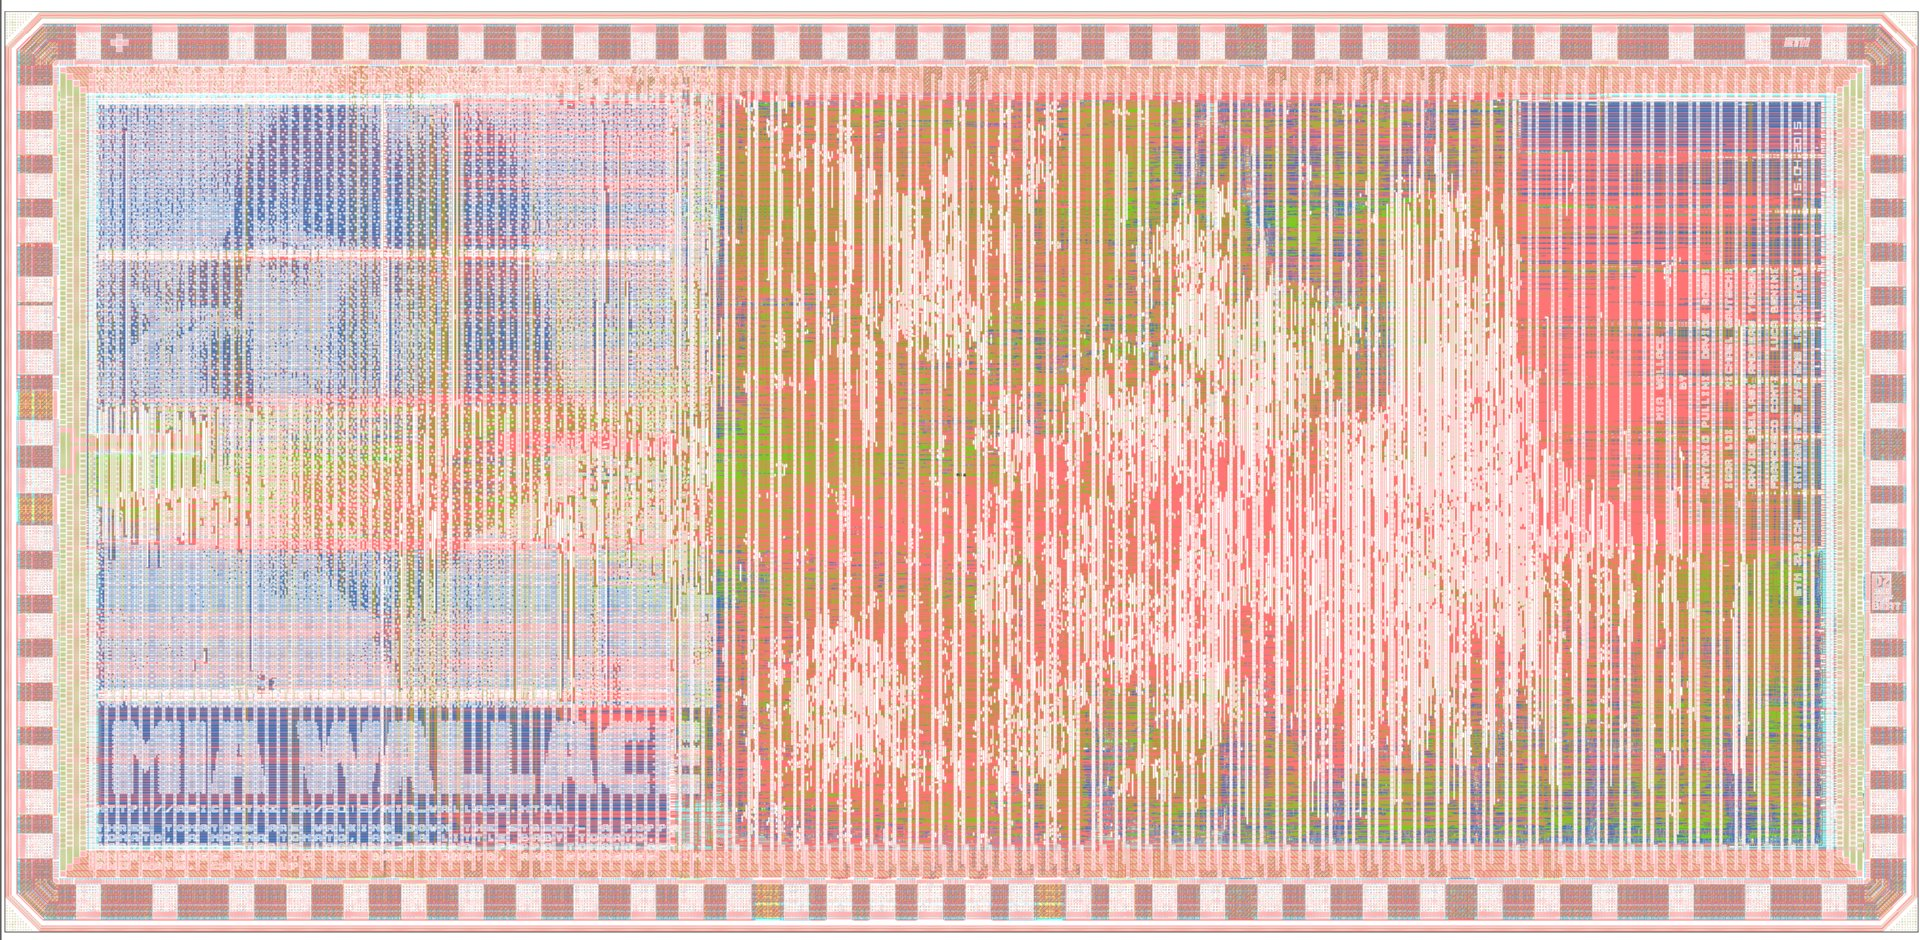
\includegraphics[width=0.7\textwidth]{figures/mia_wallace_layout_rev_sml}
  %
  \vfill
  % 
  \begin{itemize}
    \item Max. Frequency: 333 MHz @ 1.08V
    \item L2 Memory: 256 kB
    \item TCDM: 64 + 8 kB
  \end{itemize}
  % 
  \vfill
\end{frame}


\subsection{Performance}

\begin{frame}
\frametitle{Performance: MAC and Vectorial}
\framesubtitle{Increased up to 5x}
  % 
  \vfill
    \centering
    {\scriptsize
\ref{perflegend}
}

\begin{tikzpicture}[font=\scriptsize, tight background]
\begin{axis}[
  ylabel={Speedup},
  width=.56\linewidth,
  height=.50\linewidth,
  xtick=data,
  ybar=0,
  bar width=4,
  grid,
  ymin=0.4,
  ymax=1.43,
	ytick={0.4,0.5,0.6,0.7,0.8,0.9,1,1.1,1.2,1.3,1.4},
  yticklabel style={/pgf/number format/.cd,fixed,precision=2},
  every axis y label/.style={at={(ticklabel cs:.5,5)},rotate=90},
	xticklabels={aes-cbc,sha,conv2d,fft,ipm},
	cycle list name=mylist,
  enlarge x limits=0.2,
  legend to name=perflegend,
	legend style={
		draw=none,
		legend columns=2,
		/tikz/every even column/.append style={column sep=.5cm},
    transpose legend,
    legend cell align=left
	}
  ]

	\coordinate (A) at (axis cs:0,1);
	\coordinate (O1) at (rel axis cs:0,0);
	\coordinate (O2) at (rel axis cs:1,0);
	\draw [black,sharp plot,line width=1pt] (A -| O1) -- (A -| O2);
	\pgfplotsset{cycle list shift=6};
	\addplot table [x expr=\coordindex, y expr={\thisrow{cfg}/\thisrow{cfgor1200}},col sep=comma] {data/perf-lo.csv};
	\addplot table [x expr=\coordindex, y expr={\thisrow{cfg}/\thisrow{cfgGCC}},col sep=comma] {data/perf-lo.csv};
	\pgfplotsset{cycle list shift=-2};
	\addplot table [x expr=\coordindex, y expr={\thisrow{cfg}/\thisrow{cfg}},col sep=comma] {data/perf-lo.csv};
	\addplot table [x expr=\coordindex, y expr={\thisrow{cfg}/\thisrow{cfgIH}},col sep=comma] {data/perf-lo.csv};
	\addplot table [x expr=\coordindex, y expr={\thisrow{cfg}/\thisrow{cfgIHM}},col sep=comma] {data/perf-lo.csv};
	\addplot table [x expr=\coordindex, y expr={\thisrow{cfg}/\thisrow{cfgIHVM}},col sep=comma] {data/perf-lo.csv};
	\addplot table [x expr=\coordindex, y expr={\thisrow{cfg}/\thisrow{cortexM4}},col sep=comma] {data/perf-lo.csv};
	\legend{{GCC: OR1200},{GCC: OR10N},{LLVM: OR10N},{+HWLP,LD/ST},{+HWLP,LD/ST,MAC},{+HWLP,LD/ST,MAC,VEC}, {Cortex M4}};

\end{axis}
\end{tikzpicture}
%
\begin{tikzpicture}[font=\scriptsize, tight background]
\begin{axis}[
  ylabel={Speedup},
  width=.47\linewidth,
  height=.50\linewidth,
  xtick=data,
  ybar=0,
  bar width=4,
  grid,
  ymin=0.5,
  ymax=5.2,
	ytick={0,0.5,1,1.5,2,2.5,3,3.5,4,4.5,5},
  yticklabel style={/pgf/number format/.cd,fixed,precision=2},
  every axis y label/.style={at={(ticklabel cs:.5,5)},rotate=90},
	xticklabels={fir,mm8,mm16,mm32},
  %x tick label style={rotate=0,anchor=east},
	cycle list name=mylist,
  enlarge x limits=0.2,
  ]

	\coordinate (A) at (axis cs:0,1);
	\coordinate (O1) at (rel axis cs:0,0);
	\coordinate (O2) at (rel axis cs:1,0);
	\draw [black,sharp plot,line width=1pt] (A -| O1) -- (A -| O2);
	\pgfplotsset{cycle list shift=6};
	\addplot table [x expr=\coordindex, y expr={\thisrow{cfg}/\thisrow{cfgor1200}},col sep=comma] {data/perf-hi.csv};
	\addplot table [x expr=\coordindex, y expr={\thisrow{cfg}/\thisrow{cfgGCC}},col sep=comma] {data/perf-hi.csv};
	\pgfplotsset{cycle list shift=-2};
	\addplot table [x expr=\coordindex, y expr={\thisrow{cfg}/\thisrow{cfg}},col sep=comma] {data/perf-hi.csv};
	\addplot table [x expr=\coordindex, y expr={\thisrow{cfg}/\thisrow{cfgIH}},col sep=comma] {data/perf-hi.csv};
	\addplot table [x expr=\coordindex, y expr={\thisrow{cfg}/\thisrow{cfgIHM}},col sep=comma] {data/perf-hi.csv};
	\addplot table [x expr=\coordindex, y expr={\thisrow{cfg}/\thisrow{cfgIHVM}},col sep=comma] {data/perf-hi.csv};
	\addplot table [x expr=\coordindex, y expr={\thisrow{cfg}/\thisrow{cortexM4}},col sep=comma] {data/perf-hi.csv};


\end{axis}
\end{tikzpicture}
\vspace*{-1.2em}

  \vfill
\end{frame}
\note[itemize]
{
  \item Vectorial speedup alone by 2.7x
  \item IPM: Image Processing Algorithm
}

\begin{frame}
\frametitle{Performance: Bit Count}
\framesubtitle{Increased up to 35x}
  % 
  \centering
  {\scriptsize
\ref{perflegend2}
}

\hspace{5em}
\begin{tikzpicture}[font=\scriptsize, tight background]
\begin{axis}[
  ylabel={Speedup},
  width=.30\linewidth,
  height=7.5cm,
  xtick=data,
  ybar=0,
  bar width=6.5,
  grid,
  ymin=0.6,
  ymax=3.8,
	ytick={0.6,1,1.4,1.8,2.2,2.6,3.0,3.4,3.8},
  yticklabel style={/pgf/number format/.cd,fixed,precision=2},
  every axis y label/.style={at={(ticklabel cs:.5,5)},rotate=90},
	xticklabels={bitDesc.},
	cycle list name=mylist,
  enlarge x limits=0.4,
  legend to name=perflegend2,
	legend style={
		draw=none,
		legend columns=2,
		/tikz/every even column/.append style={column sep=.5cm},
    transpose legend,
    legend cell align=left
	}
  ]

	\coordinate (A) at (axis cs:0,1);
	\coordinate (O1) at (rel axis cs:0,0);
	\coordinate (O2) at (rel axis cs:1,0);
	\draw [black,sharp plot,line width=1pt] (A -| O1) -- (A -| O2);
	\addplot table [x expr=\coordindex, y expr={\thisrow{cfg}/\thisrow{cfg}},col sep=comma] {data/perf-bit.csv};
	\addplot table [x expr=\coordindex, y expr={\thisrow{cfg}/\thisrow{cfgIH}},col sep=comma] {data/perf-bit.csv};
	\pgfplotsset{cycle list shift=1};
	\addplot table [x expr=\coordindex, y expr={\thisrow{cfg}/\thisrow{cfgIHVM}},col sep=comma] {data/perf-bit.csv};
	\pgfplotsset{cycle list shift=2};
	\addplot table [x expr=\coordindex, y expr={\thisrow{cfg}/\thisrow{cfgIHVMC}},col sep=comma] {data/perf-bit.csv};
	\legend{Base,{+HWLP,LD/ST},{+HWLP,LD/ST,MAC,VEC},{+HWLP,LD/ST,MAC,VEC,BIT}};
\end{axis}
\end{tikzpicture}
\hspace{1em}
\begin{minipage}[c][0cm]{0.45\linewidth}
\vspace{45pt}
\begin{tikzpicture}[font=\scriptsize, tight background]
\begin{groupplot}[
    group style={
        group name=my fancy plots,
        group size=1 by 2,
        xticklabels at=edge bottom,
        vertical sep=0pt
    },
  width=0.7\linewidth,
  xtick=data,
  ybar=0,
  grid,
  every axis y label/.style={at={(ticklabel cs:.5,5)},rotate=90},
	xticklabels={KP Matching},
	cycle list name=mylist,
  enlarge x limits=0.4,
]
%
\nextgroupplot[ymin=30,ymax=36,
               ytick={34,35,36},
               axis x line=none, 
               axis y discontinuity=crunch,
               height=4.1cm]
	\coordinate (A) at (axis cs:0,1);
	\coordinate (O1) at (rel axis cs:0,0);
	\coordinate (O2) at (rel axis cs:1,0);
	\addplot table [x expr=\coordindex, y expr={\thisrow{cfg}/\thisrow{cfg}},col sep=comma] {data/perf-bit2.csv};
	\addplot table [x expr=\coordindex, y expr={\thisrow{cfg}/\thisrow{cfgIH}},col sep=comma] {data/perf-bit2.csv};
	\pgfplotsset{cycle list shift=1};
	\addplot table [x expr=\coordindex, y expr={\thisrow{cfg}/\thisrow{cfgIHVM}},col sep=comma] {data/perf-bit2.csv};
	\pgfplotsset{cycle list shift=2};
	\addplot table [x expr=\coordindex, y expr={\thisrow{cfg}/\thisrow{cfgIHVMC}},col sep=comma] {data/perf-bit2.csv};
%
\nextgroupplot[ymin=0,ymax=1.5,
               ytick={0,0.2,0.4,0.6,0.8,1,1.2},
               axis x line=bottom,
               height=5.0cm]
	\coordinate (A) at (axis cs:0,1);
	\coordinate (O1) at (rel axis cs:0,0);
	\coordinate (O2) at (rel axis cs:1,0);
	\draw [black,sharp plot,line width=1pt] (A -| O1) -- (A -| O2);
	\addplot table [x expr=\coordindex, y expr={\thisrow{cfg}/\thisrow{cfg}},col sep=comma] {data/perf-bit2.csv};
	\addplot table [x expr=\coordindex, y expr={\thisrow{cfg}/\thisrow{cfgIH}},col sep=comma] {data/perf-bit2.csv};
	\pgfplotsset{cycle list shift=1};
	\addplot table [x expr=\coordindex, y expr={\thisrow{cfg}/\thisrow{cfgIHVM}},col sep=comma] {data/perf-bit2.csv};
	\pgfplotsset{cycle list shift=2};
	\addplot table [x expr=\coordindex, y expr={\thisrow{cfg}/\thisrow{cfgIHVMC}},col sep=comma] {data/perf-bit2.csv};

  ylabel={Speedup},
	xticklabels={KP Matching},
	cycle list name=mylist,
\end{groupplot}
\end{tikzpicture}
\end{minipage}

\end{frame}
\note[itemize]
{
  \item Vectorial speedup alone by 2.7x
}


\subsection{Area \& Timing}

\begin{frame}
  \frametitle{Area \& Timing}
  \framesubtitle{Area increase by 25\%}
  % 
  \begin{minipage}[c][5cm]{0.58\linewidth}
    \begin{tabular}{@{}lrr@{}}
      \textbf{Feature}  & \textbf{Area}    & \\ \Xhline{2\arrayrulewidth}
      \drawbar{gray!20}   Baseline         & 35.5 kGE &         \\ \hline
      \drawbar{blue!60}   HWLP             &  3.0 kGE &  +8.5\%   \\ \hline
      \drawbar{blue!60}   Reg. File Add.   &  3.7 kGE & +10.4\%   \\ \hline
      \drawbar{red!60}    New MAC          &  1.2 kGE &  +3.3\%   \\ \hline
      \drawbar{orange!60} Vectorial ALU    &  1.9 kGE &  +5.3\%   \\ \hline
      \drawbar{green!60}  Bit Count        &  0.2 kGE &  +0.8\%   \\ \Xhline{3\arrayrulewidth}
                          \textit{Total}   & \textit{44.5 kGE} & 
    \end{tabular}
    %
    \vfill
    %
    \begin{itemize}
      \item No increase in critical path
    \end{itemize}
  \end{minipage}
  \hfill
  \begin{minipage}[c][5cm]{0.36\linewidth}
    \ref{areapowerlegend}

\hspace*{-1em}
\begin{tikzpicture}[font=\scriptsize, tight background]
\begin{axis}[
  ylabel={Area [$kGE$]},
  width=.65\linewidth,
  height=1.1\linewidth,
  ybar=0pt,
	xtick=data,
  bar width=5,
  ymin=0,
  grid,
  yticklabel style={font=\tiny,/pgf/number format/.cd,fixed,precision=1},
  every axis y label/.style={at={(ticklabel cs:.5,5)},rotate=90},
	xticklabels={Core},
	cycle list name=mylist,
  enlarge x limits=0.3,
	legend to name=areapowerlegend,
	legend style={
		draw=none,
		legend columns=1,
		/tikz/every even column/.append style={column sep=.5cm},
    transpose legend,
    legend cell align=left
  },
  ]

\addplot table [x expr=\coordindex, y=base,col sep=comma] {data/area.csv};
\addplot table [x expr=\coordindex, y=cfgIH,col sep=comma] {data/area.csv};
\addplot table [x expr=\coordindex, y=cfgIHM,col sep=comma] {data/area.csv};
\addplot table [x expr=\coordindex, y=cfgIHVM,col sep=comma] {data/area.csv};
\pgfplotsset{cycle list shift=1};
\addplot table [x expr=\coordindex, y=cfgIHVMC,col sep=comma] {data/area.csv};
%	\legend{Base,{+HWLP,LD/ST},{+HWLP,LD/ST,MAC},{+HWLP,LD/ST,MAC,VEC}};

\end{axis}
\end{tikzpicture}
\begin{tikzpicture}[font=\scriptsize, tight background]
\begin{axis}[
	ylabel near ticks,
	yticklabel pos=right,
  width=.65\linewidth,
  height=1.1\linewidth,
  ybar=0pt,
  ymin=1400,
	xtick=data,
  bar width=5,
  ymin=0,
  grid,
  yticklabel style={font=\tiny,/pgf/number format/.cd,fixed,precision=1},
  every axis y label/.style={at={(ticklabel cs:.5,5)},rotate=90},
	xticklabels={Cluster},
	cycle list name=mylist,
  enlarge x limits=0.3,
  ]

\addplot table [x expr=\coordindex, y=base,col sep=comma] {data/area-cluster.csv};
\addplot table [x expr=\coordindex, y=cfgIH,col sep=comma] {data/area-cluster.csv};
\addplot table [x expr=\coordindex, y=cfgIHM,col sep=comma] {data/area-cluster.csv};
\addplot table [x expr=\coordindex, y=cfgIHVM,col sep=comma] {data/area-cluster.csv};
\pgfplotsset{cycle list shift=1};
\addplot table [x expr=\coordindex, y=cfgIHVMC,col sep=comma] {data/area-cluster.csv};

\end{axis}
\end{tikzpicture}

  \end{minipage}
\end{frame}
\note[itemize]
{
  \item Cluster Area increased by 2.3\%
}



\subsection{Energy}

\begin{frame}
  \frametitle{Energy}
  \framesubtitle{45\% more energy efficient on average}
  % 
  \vfill
  %
  \ref{energylegend}

\begin{tikzpicture}[font=\scriptsize, tight background]
\begin{axis}[
  ylabel={Normalized Core Energy},
  width=0.55\linewidth,
  height=.5\linewidth,
  ybar=0pt,
	xtick=data,
  bar width=5,
  grid,
  ymin=0.2,
  ymax=1.3,
  ytick={0.2,0.4,0.6,0.8,1,1.2},
  yticklabel style={font=\tiny,/pgf/number format/.cd,fixed,precision=1},
  every axis y label/.style={at={(ticklabel cs:.5,5)},rotate=90},
	xticklabels={mm8, mm16, mm32, fir, fft},
	cycle list name=mylist,
  enlarge x limits=0.2,
	legend to name=energylegend,
	legend style={
		draw=none,
		legend columns=1,
		/tikz/every even column/.append style={column sep=.5cm},
    transpose legend,
    legend cell align=left
  },
  ]

	\coordinate (A) at (axis cs:0,1);
	\coordinate (O1) at (rel axis cs:0,0);
	\coordinate (O2) at (rel axis cs:1,0);
	\draw [black,sharp plot,line width=1pt] (A -| O1) -- (A -| O2);
	\addplot table [x expr=\coordindex, y=base,col sep=comma] {data/energy.csv};
	\pgfplotsset{cycle list shift=1};
	\addplot table [x expr=\coordindex, y=cfgIHM,col sep=comma] {data/energy.csv};
	\addplot table [x expr=\coordindex, y=cfgIHVM,col sep=comma] {data/energy.csv};
	%\addplot table [x expr=\coordindex, y=cortexM4,col sep=comma] {data/energy.csv};
	\legend{Base,{+HWLP,LD/ST,MAC},{+HWLP,LD/ST,MAC,VEC}};

\end{axis}
\end{tikzpicture}
\hspace{2em}
\begin{tikzpicture}[font=\scriptsize, tight background]
\begin{axis}[
  ylabel={Avg. Power [$mW$]},
  width=.25\linewidth,
  height=.5\linewidth,
  xtick=data,
  ybar=0pt,
  ymin=0,
  bar width=5,
  grid,
  yticklabel style={font=\tiny,/pgf/number format/.cd,fixed,precision=1},
  every axis y label/.style={at={(ticklabel cs:.5,5)},rotate=90},
	xticklabels={Core,1-core cluster, 4-core cluster},
  enlarge x limits=0.2,
	cycle list name=mylist,
  ]

\addplot table [x expr=\coordindex, y=base,col sep=comma] {data/power.csv};
\pgfplotsset{cycle list shift=1};
\addplot table [x expr=\coordindex, y=cfgIHM,col sep=comma] {data/power.csv};
\addplot table [x expr=\coordindex, y=cfgIHVM,col sep=comma] {data/power.csv};

\end{axis}
\end{tikzpicture}
\begin{tikzpicture}[font=\scriptsize, tight background]
\begin{axis}[
	ylabel near ticks,
	yticklabel pos=right,
  width=.25\linewidth,
  height=.5\linewidth,
  xtick=data,
  ybar=0pt,
  ymin=0,
  bar width=5,
  grid,
  yticklabel style={font=\tiny,/pgf/number format/.cd,fixed,precision=1},
  every axis y label/.style={at={(ticklabel cs:.5,5)},rotate=90},
	xticklabels={Cluster},
  enlarge x limits=0.2,
	cycle list name=mylist,
  ]

\addplot table [x expr=\coordindex, y=base,col sep=comma] {data/power-cluster.csv};
\pgfplotsset{cycle list shift=1};
\addplot table [x expr=\coordindex, y=cfgIHM,col sep=comma] {data/power-cluster.csv};
\addplot table [x expr=\coordindex, y=cfgIHVM,col sep=comma] {data/power-cluster.csv};

\end{axis}
\end{tikzpicture}
\vspace*{-0.9em}

  %
  \vfill
\end{frame}
\note[itemize]
{
  \item Cluster Power increase by 18\%
}


\section{Conclusion}

\begin{frame}
  \frametitle{Conclusion}
  \begin{itemize}
    \item Vectorial unit and new MAC cost only \textasciitilde9\% core area \\
          {\color{gray}Less than 1\% cluster area increase}
      \vfill
    \item Up to 5x speedup compared to base OpenRISC on vectorial code
          {\color{gray}Instructions can be generated automatically by the compiler}
      \vfill
    \item Up to 35x speedup with bit counting instructions
      \vfill
    \item No increase in critical path
      \vfill
    \item 45\% more energy efficient
  \end{itemize}
\end{frame}


%%%%%%%%%%%%%%%%%%%%%%%%%%%%%%%%%%%%%%%%%%%%%%%%%%%%%%%%%%%%%%%%%%%%%%

% Save the frame counter of the final frame in order to set it to this
% value at the beginning of the backup slides (because I do not want
% to count the empty slide between the main content slides and the
% backup slides).
\newcounter{finalframe}
\setcounter{finalframe}{\value{framenumber}}

% Start the appendix in order to start a new navigation hierarchy for
% the backup slides on the top of the slides (different to that of the
% actual main content slides).
\appendix

% Start of the backup slides.
\beginbackup

%%%%%%%%%%%%%%%%%%%%%%%%%%%%%%%%%%%%%%%%%%%%%%%%%%%%%%%%%%%%%%%%%%%%%%
%%%%% Start of Frame
\begin{frame}[plain]
  % Insert an empty slide in order to separate the main content slides
  % from the backup slides.
\end{frame}
%%%%%%%%%%%%%%%%%%%%%%%%%%%%%%%%%%%%%%%%%%%%%%%%%%%%%%%%%%%%%%%%%%%%%%

% Set the counter of the first backup slide to the next number after
% the last main content slide number (do not count the empty slide
% between the main content slides and the backup slides).
\setcounter{framenumber}{\value{finalframe}}


%%%%%%%%%%%%%%%%%%%%%%%%%%%%%%%%%%%%%%%%%%%%%%%%%%%%%%%%%%%%%%%%%%%%%%
%%%%% Start of Frame
\begin{frame}[plain]
  \frametitle{Backup Slides}
\end{frame}
%%%%%%%%%%%%%%%%%%%%%%%%%%%%%%%%%%%%%%%%%%%%%%%%%%%%%%%%%%%%%%%%%%%%%%



\begin{frame}
  \frametitle{Outlook}
  \begin{itemize}
    \item Look into fractional support \\
      {\color{gray}$rD = (rD \gg 16) + (rA[31:16] \cdot rB[31:16]) \ll 1$}
    \item Redesign multiplier \\
      \vfill
      \begin{center}
        \includegraphics[width=0.8\textwidth]{figures/outlook_mul}
      \end{center}
  \end{itemize}
\end{frame}


\begin{frame}
\frametitle{Performance: MAC and Vectorial}
\framesubtitle{Increased up to 5x}
  % 
  \vfill
    \centering
    {\scriptsize
\ref{perflegend_bckp}
}

\begin{tikzpicture}[font=\scriptsize, tight background]
\begin{axis}[
  ylabel={Speedup},
  width=.56\linewidth,
  height=.50\linewidth,
  xtick=data,
  ybar=0,
  bar width=4.5,
  grid,
  ymin=0.6,
  ymax=1.43,
	ytick={0.6,0.7,0.8,0.9,1,1.1,1.2,1.3,1.4},
  yticklabel style={/pgf/number format/.cd,fixed,precision=2},
  every axis y label/.style={at={(ticklabel cs:.5,5)},rotate=90},
	xticklabels={aes-cbc,sha,conv2d,fft,ipm},
	cycle list name=mylist,
  enlarge x limits=0.2,
  legend to name=perflegend_bckp,
	legend style={
		draw=none,
		legend columns=-1,
		/tikz/every even column/.append style={column sep=.5cm},
		at={(1.0,1.4)}
	}
  ]

	\coordinate (A) at (axis cs:0,1);
	\coordinate (O1) at (rel axis cs:0,0);
	\coordinate (O2) at (rel axis cs:1,0);
	\draw [black,sharp plot,line width=1pt] (A -| O1) -- (A -| O2);
	\addplot table [x expr=\coordindex, y expr={\thisrow{cfg}/\thisrow{cfg}},col sep=comma] {data/perf-lo.csv};
	%\pgfplotsset{cycle list shift=1};
	\addplot table [x expr=\coordindex, y expr={\thisrow{cfg}/\thisrow{cfgIH}},col sep=comma] {data/perf-lo.csv};
	\addplot table [x expr=\coordindex, y expr={\thisrow{cfg}/\thisrow{cfgIHM}},col sep=comma] {data/perf-lo.csv};
	\addplot table [x expr=\coordindex, y expr={\thisrow{cfg}/\thisrow{cfgIHVM}},col sep=comma] {data/perf-lo.csv};
	\addplot table [x expr=\coordindex, y expr={\thisrow{cfg}/\thisrow{cortexM4}},col sep=comma] {data/perf-lo.csv};
	\legend{Base,+IH,+IHM,+IHVM,Cortex-M4};

\end{axis}
\end{tikzpicture}
%
\begin{tikzpicture}[font=\scriptsize, tight background]
\begin{axis}[
  ylabel={Speedup},
  width=.47\linewidth,
  height=.50\linewidth,
  xtick=data,
  ybar=0,
  bar width=4.5,
  grid,
  ymin=0.5,
  ymax=5.2,
	ytick={0,0.5,1,1.5,2,2.5,3,3.5,4,4.5,5},
  yticklabel style={/pgf/number format/.cd,fixed,precision=2},
  every axis y label/.style={at={(ticklabel cs:.5,5)},rotate=90},
	xticklabels={fir,mm8,mm16,mm32},
  %x tick label style={rotate=0,anchor=east},
	cycle list name=mylist,
  enlarge x limits=0.2,
  ]

	\coordinate (A) at (axis cs:0,1);
	\coordinate (O1) at (rel axis cs:0,0);
	\coordinate (O2) at (rel axis cs:1,0);
	\draw [black,sharp plot,line width=1pt] (A -| O1) -- (A -| O2);
	\addplot table [x expr=\coordindex, y expr={\thisrow{cfg}/\thisrow{cfg}},col sep=comma] {data/perf-hi.csv};
	%\pgfplotsset{cycle list shift=1};
	\addplot table [x expr=\coordindex, y expr={\thisrow{cfg}/\thisrow{cfgIH}},col sep=comma] {data/perf-hi.csv};
	\addplot table [x expr=\coordindex, y expr={\thisrow{cfg}/\thisrow{cfgIHM}},col sep=comma] {data/perf-hi.csv};
	\addplot table [x expr=\coordindex, y expr={\thisrow{cfg}/\thisrow{cfgIHVM}},col sep=comma] {data/perf-hi.csv};
	\addplot table [x expr=\coordindex, y expr={\thisrow{cfg}/\thisrow{cortexM4}},col sep=comma] {data/perf-hi.csv};

\end{axis}
\end{tikzpicture}
\vspace*{-1.2em}

  \vfill
\end{frame}

\begin{frame}
  \frametitle{Area Multiplier}
  \framesubtitle{in 28nm}
  % 
  \small
  \centering\begin{tabular}{@{}llrrr@{}} \hline
    \textbf{Design}      & \textbf{Features} & \textbf{Area OR10N} & \textbf{Area Mult.} & \textbf{Timing} \\ \hline
    Baseline             &                   &             $20125$ &              $5950$ &       $7.57$ ns \\
    Vec. Booth Mult.     & MAC               &             $18925$ &              $5230$ &       $7.83$ ns \\
    Vec. Booth Mult.     & MAC, subword      &             $18850$ &              $5451$ &       $7.83$ ns \\
    Shared Segmentation  & MAC               &             $19518$ &              $6687$ &       $7.77$ ns \\
    Shared Segmentation  & MAC, subword      &             $18854$ &              $5125$ &       $7.84$ ns \\
    Behavioral           & MAC               &             $18900$ &              $4202$ &       $7.58$ ns \\
    Behavioral           & MAC, subword      &             $18884$ &              $4287$ &       $7.64$ ns \\
    \hline
  \end{tabular}
  %
\end{frame}

\begin{frame}
\frametitle{Vectorial Booth Multiplier}
  % 
  \vfill
    \centering
    \centering\includegraphics[height=0.80\textwidth,angle=270]{figures/booth_mult}
  \vfill
\end{frame}

% End of backup slides.
\backupend

%%%%%%%%%%%%%%%%%%%%%%%%%%%%%%%%%%%%%%%%%%%%%%%%%%%%%%%%%%%%%%%%%%%%%%
%%%%%                                                                %
%%%%% Document End                                                   %
%%%%%                                                                %
%%%%%%%%%%%%%%%%%%%%%%%%%%%%%%%%%%%%%%%%%%%%%%%%%%%%%%%%%%%%%%%%%%%%%%
\end{document}

